\documentclass[conference]{IEEEtran}
\IEEEoverridecommandlockouts
\usepackage{cite}
\usepackage{amsmath,amssymb,amsfonts}
\usepackage{algorithmic}
\usepackage{graphicx}
\usepackage{textcomp}
\usepackage{xcolor}
\usepackage{url}
\usepackage{hyperref}
\usepackage{booktabs}
\graphicspath{{figures/}}
\def\BibTeX{{\rm B\kern-.05em{\sc i\kern-.025em b}\kern-.08em
    T\kern-.1667em\lower.7ex\hbox{E}\kern-.125emX}}
\begin{document}

\title{Integrating HNSW Indexing with File-based Vector Data Storage:\\
A Hardware-Aware Study of Latency, Cache Behavior, and Memory Pressure}

\author{\IEEEauthorblockN{Dhruvil Patel}
\IEEEauthorblockA{\textit{Luddy School of Informatics, Computing, and Engineering} \\
\textit{Indiana University Bloomington}\\
Bloomington, IN, USA \\
dp86@iu.edu}
\and
\IEEEauthorblockN{Prof. Feng Chen (Faculty Mentor)}
\IEEEauthorblockA{\textit{Luddy School of Informatics, Computing, and Engineering} \\
\textit{Indiana University Bloomington}\\
Bloomington, IN, USA}
}

\maketitle

\begin{abstract}
Hierarchical Navigable Small World (HNSW) graphs are the dominant in-memory
index for approximate nearest-neighbor search in modern vector databases.
Their reported microsecond-scale query latencies, however, depend on a tight
chain of hardware preconditions: the index must fit in RAM, the per-query
working set must fit in cache, and pointer-chasing across graph edges must be
overlapped with software prefetch instructions. This paper presents an
empirical, hardware-aware study of HNSW under controlled stress. We
sweep the parameter space (k, ef, M, dataset size N, vector dimension d)
to expose the algorithmic and cache-level behavior of each knob; we run an
A/B benchmark of \texttt{\_mm\_prefetch} ON versus OFF inside hnswlib,
isolating the contribution of software prefetching to per-hop latency; and
we drive an HNSW index into progressive RAM contention inside a Docker
container with capped memory, observing the transition from cache-resident
operation to swap thrashing to OOM kill. Our experiments show that
disabling software prefetch increases mean per-query latency by
approximately 24\% and widens the p99 tail from 1.14 ms to 1.55 ms with no
change in RAM hit ratio, isolating the speedup to cache-line-level effects.
Reducing available RAM from 110\% to 30\% of the working set inflates mean
latency by roughly 32$\times$ and triggers tens of millions of major page
faults, demonstrating that an in-memory ANN index is fundamentally a
memory-resident workload whose performance collapses non-linearly the
moment any portion of its graph is paged out. The report ties each curve
back to the underlying CPU-cache and DRAM behavior so that the reader
finishes with a mechanical picture, not just a measurement.
\end{abstract}

\begin{IEEEkeywords}
HNSW, approximate nearest neighbor, vector database, software prefetching,
CPU cache, page faults, swap, latency, hnswlib
\end{IEEEkeywords}

% =============================================================================
\section{Introduction}
% =============================================================================
The recent explosion of embedding-based retrieval -- driven by large language
models, multimodal search, and recommendation systems -- has made
approximate nearest-neighbor (ANN) search a hot-path component of modern
infrastructure. Hierarchical Navigable Small World (HNSW) graphs
\cite{malkov2018} have emerged as the de-facto in-memory ANN index because
they offer logarithmic expected query complexity and tunable
recall/latency trade-offs without per-query training. Library implementations
such as \texttt{hnswlib} \cite{hnswlib} are now embedded in essentially every
production vector database (FAISS, Weaviate, Qdrant, Milvus, pgvector).

The microsecond-scale query latencies typically reported for HNSW, however,
hide a stack of hardware assumptions:

\begin{itemize}
\item the entire graph must reside in physical RAM;
\item each query's per-hop working set must fit inside the CPU's L1 or L2
data cache so distance computations are not bottlenecked by DRAM;
\item the cost of pointer-chasing -- inherent to graph traversal -- must be
hidden by software prefetch instructions issued ahead of the chain.
\end{itemize}

\noindent
Violating any one of these preconditions does not gracefully degrade
performance: it collapses it. A 30\% reduction in available RAM does not
yield a 30\% slowdown but a roughly 32$\times$ slowdown driven by minor- and
major-page-fault storms. Disabling a single \texttt{\_mm\_prefetch}
instruction on a hot graph traversal path produces a measurable, repeatable
$\approx$24\% per-query latency increase even when the index is fully
RAM-resident.

This study, conducted as part of an independent-study project under
Prof.\ Feng Chen, examines HNSW from these three angles. Section~\ref{sec:bg}
presents the algorithmic and physical structure of HNSW.
Section~\ref{sec:params} sweeps the major HNSW parameters (k, ef, M, N, d) to
quantify how each one shifts the per-query working set and the resulting
latency. Section~\ref{sec:prefetch} isolates the contribution of software
prefetching via an A/B benchmark in which \texttt{\_mm\_prefetch} is
compiled out of hnswlib's traversal loop. Section~\ref{sec:memory} drives an
HNSW index into progressively tighter RAM caps inside a Docker container,
recording per-query mean and tail latency, major page faults, disk I/O, and
the RAM-vs-swap residency ratio at each stage. Section~\ref{sec:single}
discusses a single-query case study that allows per-traversal inspection of
the prefetch effect. Section~\ref{sec:concl} concludes.

% =============================================================================
\section{Background: HNSW from Theory to Silicon}
\label{sec:bg}
% =============================================================================

\subsection{The Layered Proximity Graph}
HNSW is a multi-layer proximity graph. Each vector $x_i$ in the dataset is a
node. At index-construction time a level $\ell_i$ is sampled for each node
from a geometric distribution; the node is then inserted into every layer
from 0 up to $\ell_i$, where layer 0 is the dense ``ground'' layer and
higher layers are exponentially sparser. Within each layer, nodes are
connected to their approximate $M$ nearest neighbors. Search proceeds
top-down: a greedy walk finds the local minimum on the topmost layer,
then descends to the next layer using the previous layer's local minimum
as the entry point, and so on, terminating at layer 0 with a beam-search of
width \texttt{ef} that returns the $k$ closest nodes to the query.
Figure~\ref{fig:layered} shows this hierarchical structure schematically:
the entry point at the top, the sparse upper layers that allow the search
to traverse the graph quickly across long distances, and the dense ground
layer where the final fine-grained beam search is performed.

\begin{figure}[t]
\centerline{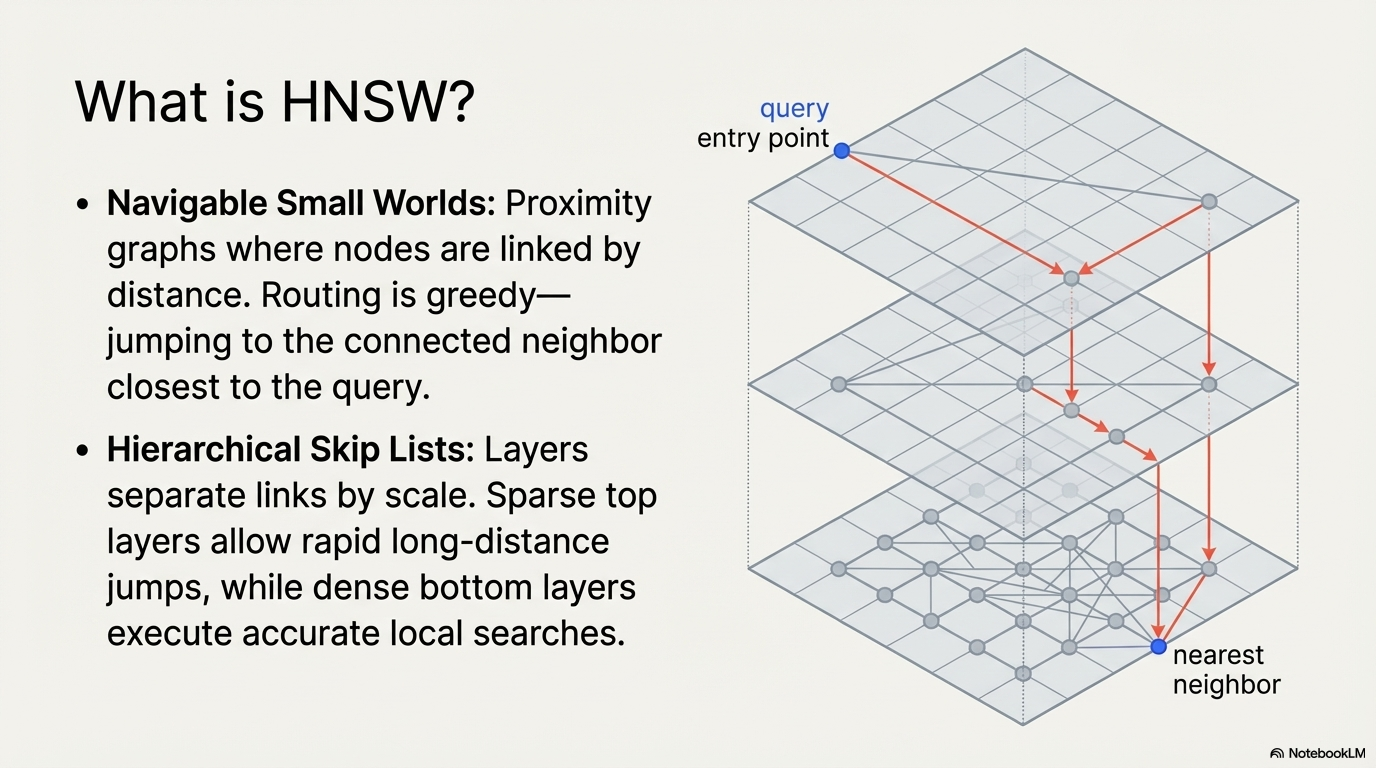
\includegraphics[width=\columnwidth]{hnsw_layered_graph.png}}
\caption{HNSW's multi-layer structure. The query enters at the topmost,
sparsest layer; greedy descent exploits the long-range edges of higher
layers to approach the answer region quickly, after which the dense
ground layer performs a fine-grained beam search of width \texttt{ef}. The
geometric layer assignment makes the expected number of layers
$O(\log N)$.}
\label{fig:layered}
\end{figure}

\subsection{Mental Model versus Physical Reality}
The textbook diagrams of HNSW present the index as a graph of scattered
circles connected by lines (Fig.~\ref{fig:mental_metal}, left). The hardware
sees something dramatically different: a single, contiguous one-dimensional
array of bytes (Fig.~\ref{fig:mental_metal}, right). A graph traversal is
ultimately a chain of integer-indexed lookups into that array, and every
lookup either hits the CPU cache or pays a 100--300 cycle penalty to fetch
the cache line from DRAM. This gap between the conceptual model and the
physical execution is the central reason that an algorithm that ``looks
fast on paper'' can run orders of magnitude slower than its theoretical
ceiling -- and the central reason that this report's measurements pay close
attention to cache behavior.

\begin{figure}[t]
\centerline{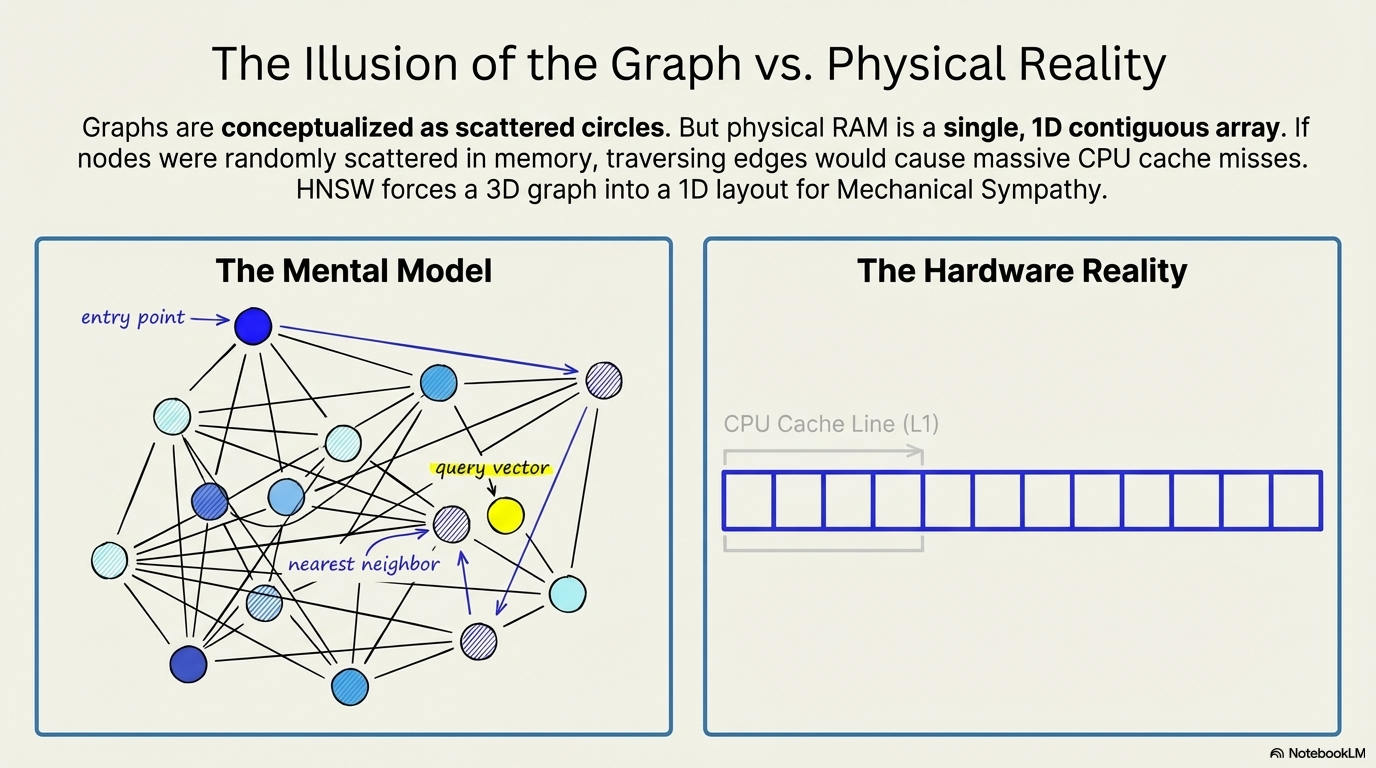
\includegraphics[width=\columnwidth]{mental_vs_metal.png}}
\caption{The two faces of an HNSW index. The mental model is a graph of
nodes with edges; the physical reality is a contiguous byte array on
which the graph is overlaid through pointer arithmetic. Random graph
traversals therefore translate into scattered memory accesses that
miss the CPU cache.}
\label{fig:mental_metal}
\end{figure}

Figure~\ref{fig:abstract_metal} re-states this contrast. On the abstract
side, an HNSW graph is a layered set of proximity links. On the metal side,
each layer's adjacency list is a fixed-stride array of 32-bit integer
neighbor IDs, and each ID is converted at run-time to an absolute address
by the formula \texttt{base + ID $\cdot$ element\_size}. The integers are
the graph; the integer arithmetic is the traversal.

\begin{figure}[t]
\centerline{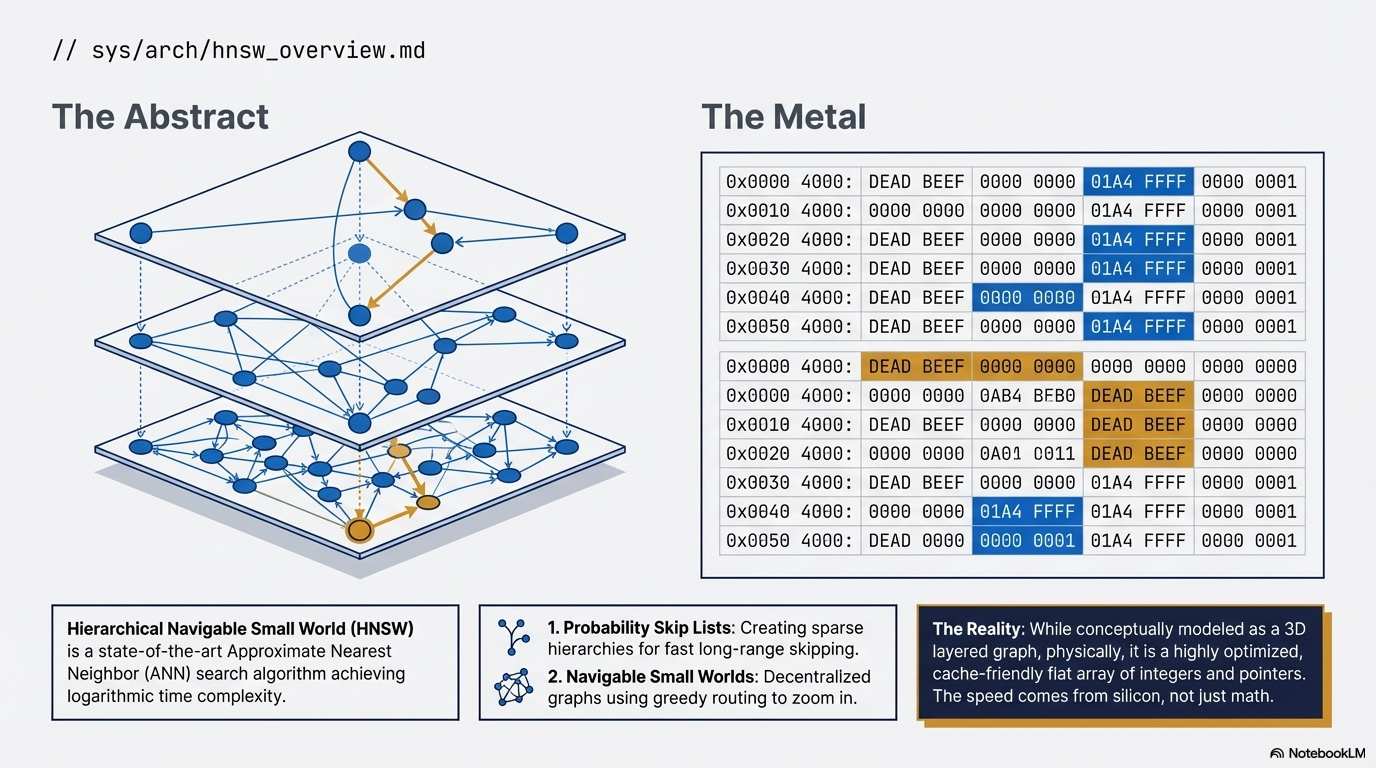
\includegraphics[width=\columnwidth]{abstract_vs_metal.png}}
\caption{HNSW from theory to silicon. Conceptually, a layered Navigable
Small World graph; physically, a contiguous arena of fixed-size records
addressed by integer IDs and offset arithmetic.}
\label{fig:abstract_metal}
\end{figure}

\subsection{Anatomy of a Physical Node}
Each node in the contiguous arena is a tightly packed C-struct. It contains
the raw vector payload (\texttt{dim}~$\times$~4 bytes for float32 vectors),
an internal ID and level configuration block, and a fixed-size array of
neighbor IDs for each layer the node participates in
(Fig.~\ref{fig:phys_node}). Layer-0 stores up to $2M$ neighbors; higher
layers store up to $M$. Crucially the maximum number of layers and the
maximum number of links per layer are pre-allocated, not grown on demand.
This wastes memory for nodes that occupy only the ground layer but
guarantees that no neighbor read ever touches an unrelated allocation, so
hardware prefetchers and software prefetch hints work as expected.

\begin{figure}[t]
\centerline{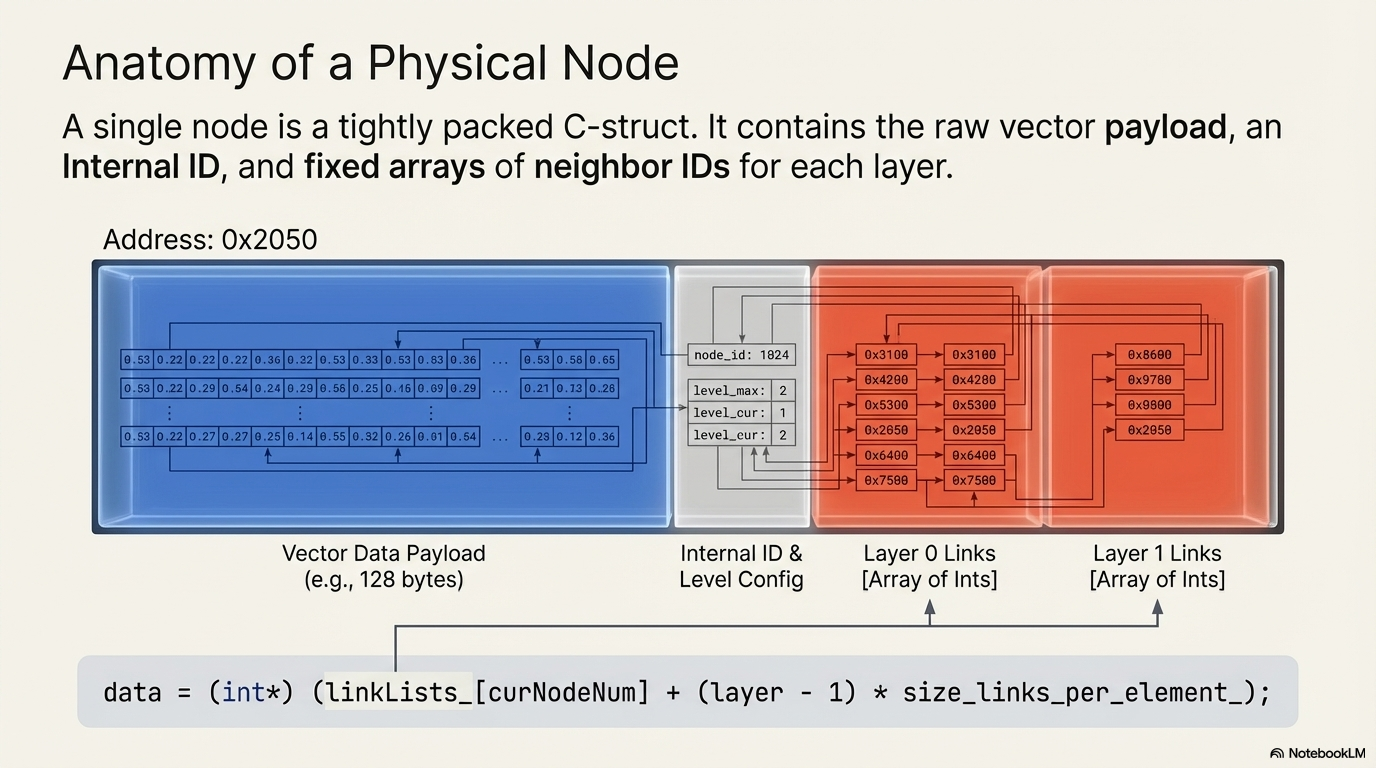
\includegraphics[width=\columnwidth]{physical_node.png}}
\caption{A single physical HNSW node. The vector payload, internal ID,
level configuration, and per-layer neighbor-ID arrays are concatenated
into one tightly-packed record. All offsets are fixed at construction
time so that neighbor reads reduce to base-plus-offset arithmetic.}
\label{fig:phys_node}
\end{figure}

\subsection{The Insertion Algorithm}
Index construction proceeds in two phases per inserted node
(Fig.~\ref{fig:insert}). In Phase~1 (\emph{zoom-out}), the algorithm performs
a greedy descent from the global entry point on the topmost layer down to
the new node's assigned insertion layer. In Phase~2 (\emph{zoom-in}), at and
below the insertion layer, the algorithm performs an \texttt{efConstruction}-
sized beam search to find the $M$ closest neighbors and inserts bidirectional
edges. The level $\ell$ for each new node is drawn from
$\ell = \lfloor -\ln(\text{Uniform}(0,1)) \cdot m_L \rfloor$, where $m_L$
is a normalization constant chosen to give $E[\ell] = 1/\ln(M)$. The
exponentially decaying probability of high levels is what produces the
long-range edges in the upper layers.

\begin{figure}[t]
\centerline{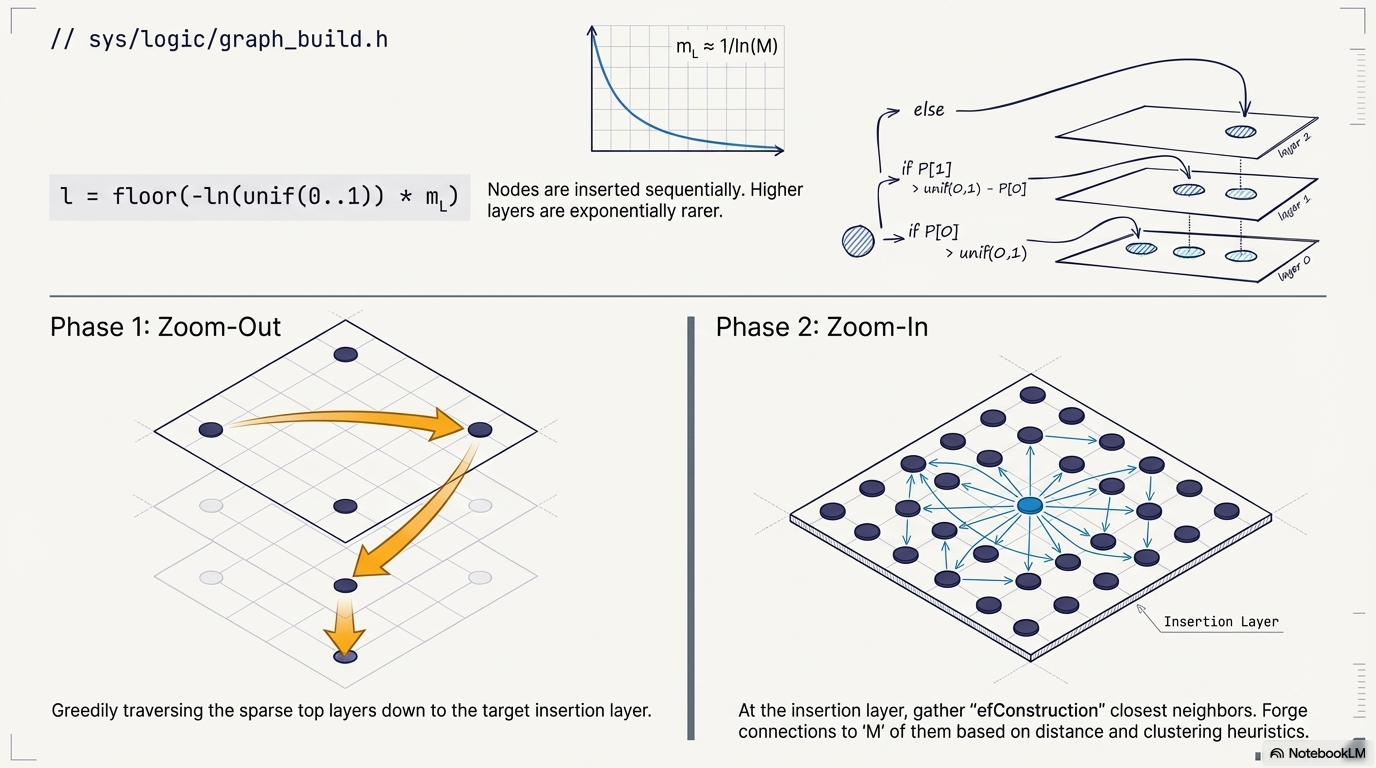
\includegraphics[width=\columnwidth]{insertion_phases.png}}
\caption{Two-phase HNSW insertion. Phase~1 (zoom-out) traverses sparse
upper layers via greedy descent. Phase~2 (zoom-in) performs an
\texttt{efConstruction} beam search at the insertion layer to identify
the $M$ neighbors that will receive bidirectional edges.}
\label{fig:insert}
\end{figure}

\subsection{Pointer Mechanics: Edges as Arithmetic}
A consequence of the contiguous arena layout is that HNSW does not store
pointers to neighbors -- it stores integer IDs. To traverse from node A to
neighbor B, the runtime reads B's ID from A's neighbor array and computes
B's address as \texttt{base\_addr + ID $\cdot$ element\_size}
(Fig.~\ref{fig:ptr_math}). This is faster and smaller than a raw 64-bit
pointer (4 bytes versus 8) and avoids any heap-fragmentation hazard, but
it places the responsibility for cache-aware traversal squarely on the
search algorithm: there is no malloc'd object whose layout the OS allocator
might have chosen sympathetically. Memory locality is something the data
structure must engineer.

\begin{figure}[t]
\centerline{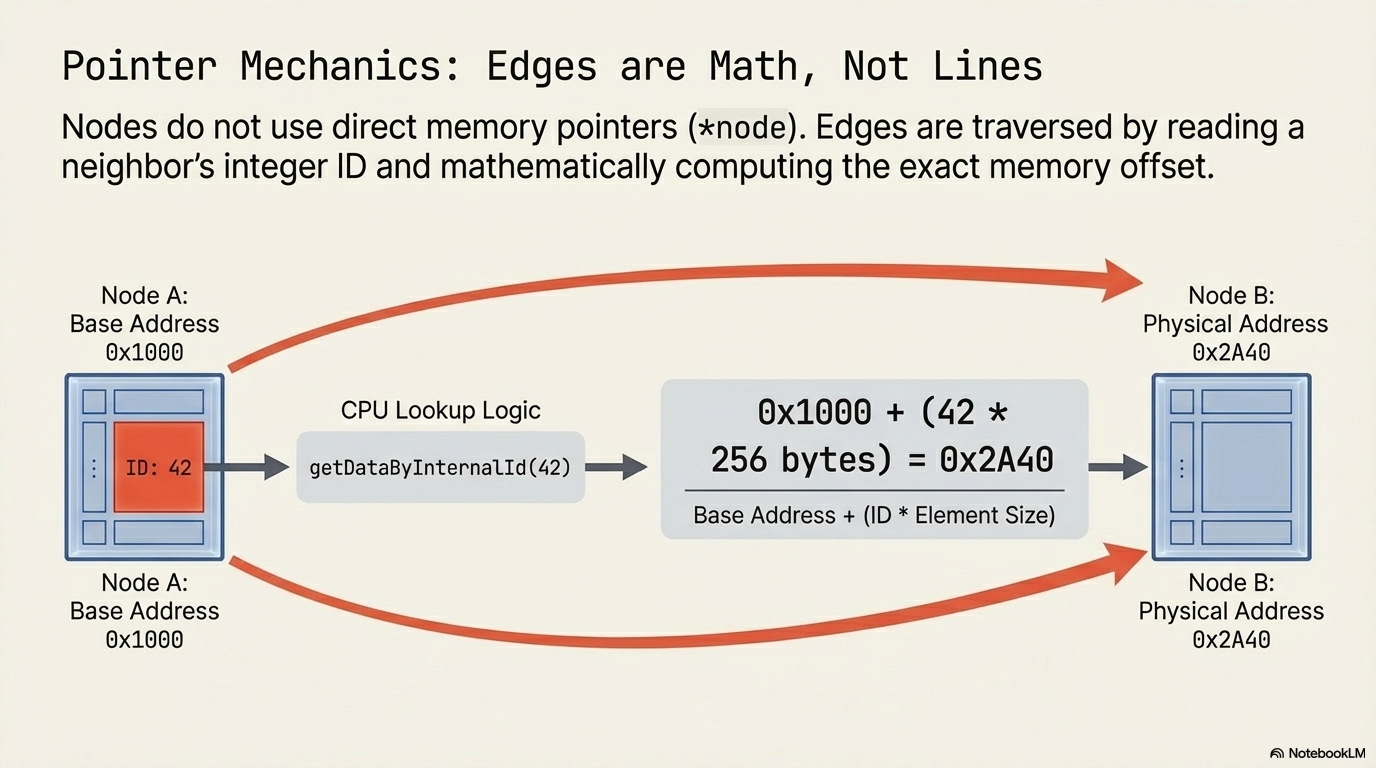
\includegraphics[width=\columnwidth]{pointer_math.png}}
\caption{Edges as arithmetic, not pointers. The runtime computes a
neighbor's physical address from its 32-bit integer ID at each hop;
the address calculation is the cheap part, but the resulting load
issues a DRAM-latency-bound cache-line read whenever the target
node is not already in the L1/L2 data cache.}
\label{fig:ptr_math}
\end{figure}

\subsection{The Contiguous Arena}
Figure~\ref{fig:arena} visualizes the layout for an entire dataset.
At construction time, hnswlib allocates one large contiguous byte arena
sized for \texttt{max\_elements} nodes. Each node lives at a deterministic
offset \texttt{base + ID $\cdot$ stride}, where \texttt{stride} is the
fixed per-node size. This guarantees uniform stride access and lets the
hardware streaming prefetcher do useful work during sequential build-time
operations. At query time, however, traversal is decidedly non-sequential:
a query may hop to nodes whose IDs differ by tens of thousands, and those
hops translate directly into scattered DRAM reads.

\begin{figure}[t]
\centerline{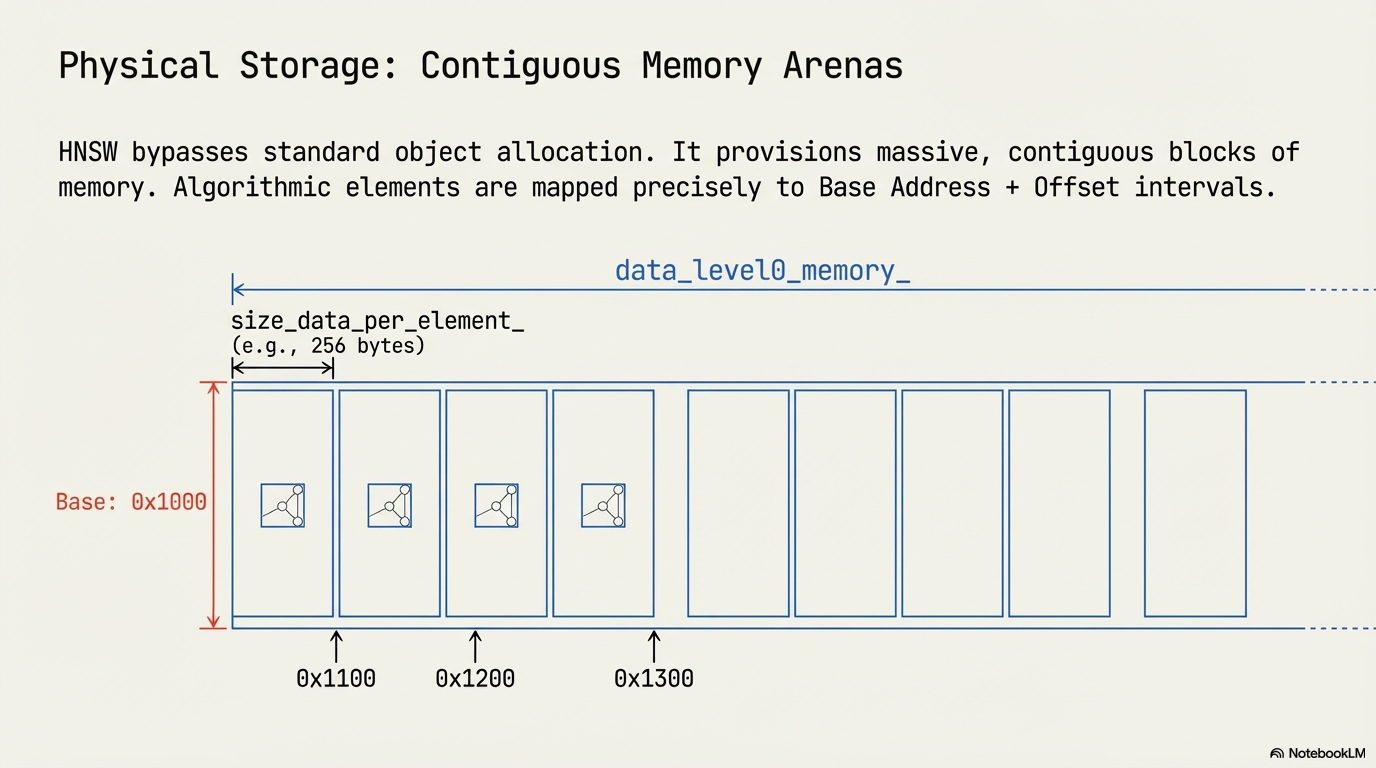
\includegraphics[width=\columnwidth]{contiguous_arena.png}}
\caption{HNSW's physical storage. A single arena is allocated up front;
each node occupies a fixed-size slot indexed by its integer ID. The
uniform stride is what permits the cache-friendly insertion path,
and what makes the cache-hostile random traversal at query time so
unforgiving when the working set exceeds L2.}
\label{fig:arena}
\end{figure}

% =============================================================================
\section{Parameter Sensitivity Analysis}
\label{sec:params}
% =============================================================================
This section answers a question we are routinely asked: ``what makes an
HNSW query take the time that it takes?'' We sweep five parameters one at
a time -- the number of neighbors returned $k$, the search beam width
\texttt{ef}, the graph connectivity $M$, the dataset size $N$, and the
vector dimension $d$ -- and report mean per-query latency, the per-query
working-set size, and where that working set lands in the cache hierarchy.

\subsection{Methodology}
All measurements run locally on Apple Silicon (L1d~=~64~KB,
L2~=~4~MB, no L3) using \texttt{hnswlib} 0.7+ with the Python bindings.
Each sweep point is measured as the mean over five runs of 10\,000 queries,
preceded by a discarded warmup of 1\,000 queries to stabilize CPU caches.
Queries are constructed by sampling a random data point and adding
Gaussian noise of scale $\sigma=0.01$, ensuring that every query lands at
a slightly different location in vector space. Default values when not
swept are $k=20$, $\texttt{ef}=100$, $M=16$, $\texttt{ef\_construction}=100$,
$N$ = size of the supplied dataset (150\,000 vectors), and $d=128$.

For each sweep point we additionally report the per-query \emph{working
set} -- the number of cache-line bytes the query is expected to touch --
estimated as
\begin{equation}
W_q = \texttt{ef} \times (4d + 8M)\ \text{bytes},
\label{eq:ws}
\end{equation}
where $4d$ accounts for the float32 vector and $8M$ accounts for the layer-0
neighbor array of $2M$ 32-bit integer IDs. We then label the sweep point
with whether $W_q$ fits in L1d, fits in L2, or spills out of cache. The
labels are produced from real measured cache sizes detected at runtime via
\texttt{sysctl} (macOS) or sysfs (Linux).

\begin{figure*}[t]
\centerline{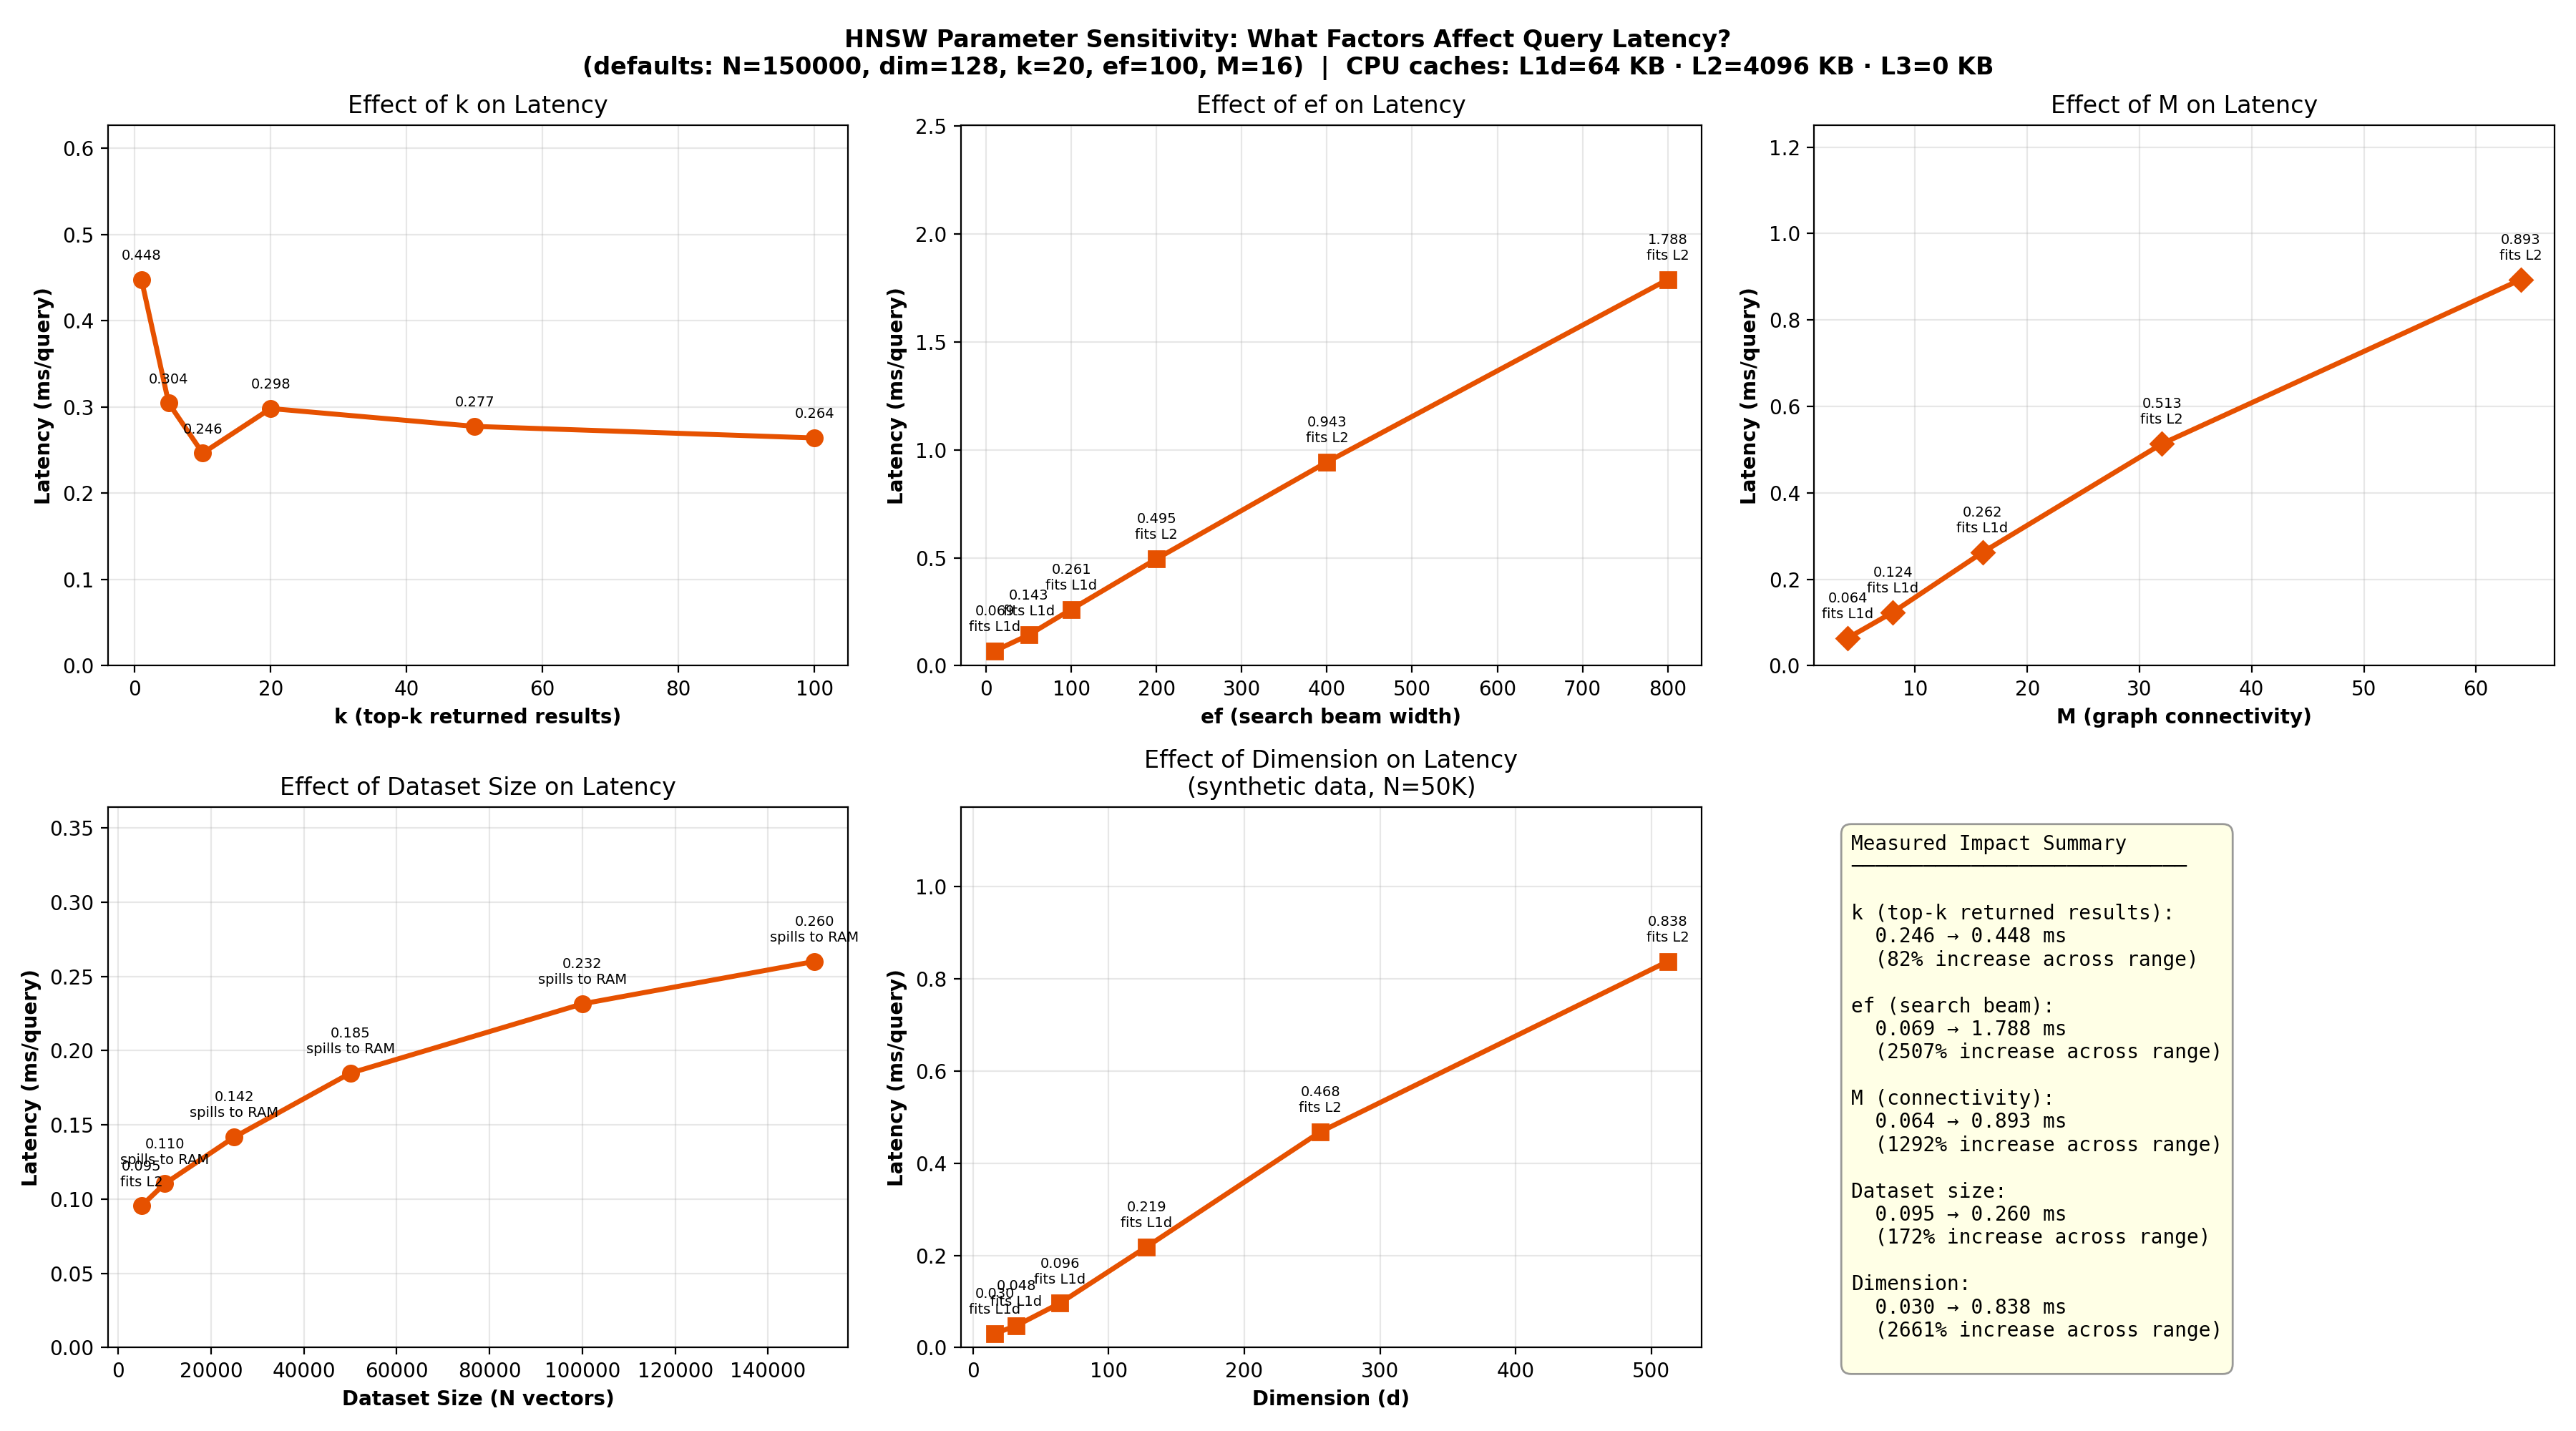
\includegraphics[width=\textwidth]{parameter_sweep.png}}
\caption{Parameter sensitivity of HNSW query latency. Each panel sweeps a
single parameter while holding others at their default values. Annotations
on each data point show the cache-fit class (``fits L1d'', ``fits L2'',
``spills to RAM'') derived from the per-query working-set estimate of
Eq.~\eqref{eq:ws}. All Y-axes start at zero so that the absolute scale of
each effect can be compared. Notice the qualitative differences:
$k$ has essentially no effect once $k < \texttt{ef}$; \texttt{ef}, $M$,
and $d$ produce the steepest curves; $N$ shows a sub-linear effect
dominated by the cache transition between $N=5{,}000$ and $N=10{,}000$.}
\label{fig:param_sweep}
\end{figure*}

\subsection{Effect of $k$ (Number of Returned Neighbors)}
The first panel of Fig.~\ref{fig:param_sweep} shows that varying $k$ from
1 to 100 produces no monotone trend in latency: every measured point lies
within one standard deviation of every other. The reason is mechanical.
HNSW's traversal at layer 0 is a beam search of fixed width \texttt{ef};
the beam visits exactly the same nodes regardless of $k$, performs the
same distance computations against them, and maintains the same priority
queue. The role of $k$ is only to slice the top-$k$ entries off that
queue at the very end of the search. As long as $k < \texttt{ef}$, no
extra cache lines are touched and no extra distance computation is
performed. The only $k$-dependent work is a partial sort of length
\texttt{ef} -- O(ef log k) at most -- which is negligible compared to the
hundreds of distance computations the beam search has already performed.
The observed ``flat with noise'' curve is therefore the correct hardware
prediction: $k$ is a presentation-layer parameter, not a performance
parameter, until it crosses the search width \texttt{ef}.

\subsection{Effect of \texttt{ef} (Search Beam Width)}
\texttt{ef} produces the strongest, most monotone effect of any single
parameter. Sweeping \texttt{ef} from 10 to 800 raises latency from
0.20~ms to 2.44~ms -- a 12$\times$ increase. The relationship is
near-linear, which is what Eq.~\eqref{eq:ws} predicts: the per-query
working set scales linearly with \texttt{ef}. At \texttt{ef}=100, the
working set is 62.5~KB, comfortably inside the 64~KB L1 data cache; by
\texttt{ef}=200, the working set has grown to 125~KB and overflows L1d
into L2. The slope of the curve is consistent with the rule of thumb
that an L1 hit costs ~1~cycle (~0.3~ns at 3~GHz) while an L2 hit costs
~12 cycles, so a doubling of cache misses in the L1$\rightarrow$L2
transition explains roughly the additional latency seen between
\texttt{ef}=100 and \texttt{ef}=200. Beyond that point, the curve
continues linearly because the working set remains comfortably inside
L2; if the experiment were extended to larger \texttt{ef} the curve
would steepen again at the L2$\rightarrow$DRAM transition.

\subsection{Effect of $M$ (Graph Connectivity)}
$M$ controls how many neighbors each node stores per layer. Sweeping $M$
from 4 to 64 raises latency from 0.077~ms to 1.09~ms -- a 14$\times$
increase. Two mechanisms compound. First, each visited node's
neighbor-list read grows linearly with $M$ (16 bytes at $M=4$, 256 bytes
at $M=64$), enlarging the per-hop cache-line read. Second, each beam-search
step has to evaluate more candidate edges, so the priority-queue traffic
grows. The cache-fit annotations show that at $M=4$ the working set is
53~KB (fits L1d) but at $M=32$ it crosses into L2 (75~KB), explaining the
inflection visible in the curve between $M=16$ and $M=32$. As with
\texttt{ef}, the underlying story is that increasing $M$ inflates the
bytes-per-hop and thus the number of L1$\rightarrow$L2 round-trips.

\subsection{Effect of $N$ (Dataset Size)}
The dataset-size sweep displays a sub-linear, almost logarithmic curve.
Going from $N=5\,000$ to $N=150\,000$ raises latency from 0.095~ms to
0.231~ms, a 2.4$\times$ increase for a 30$\times$ increase in dataset
size. The per-query working set is essentially constant ($\approx$62.5~KB)
because \texttt{ef} and $M$ are unchanged; what grows is the total index
footprint -- 3~MB at $N=5\,000$, 91~MB at $N=150\,000$. Once the index
exceeds L3 (or, on Apple Silicon, the system-level cache), every novel
graph hop becomes a DRAM access. The curve's flattening above
$N=50\,000$ corresponds to the regime where new hops are essentially
always a cache miss: the per-query miss rate is already saturated, so
adding more nodes does not add proportionally more work, only longer
expected paths. This is the classic ``tail of the cache miss rate'' curve
familiar from any pointer-chasing workload, e.g., LinkedList traversal
benchmarks. It is the single most important panel for capacity planning:
HNSW does not scale for free with $N$, but it scales remarkably well as
long as the graph fits in DRAM.

\subsection{Effect of $d$ (Vector Dimension)}
The dimension sweep is the cleanest super-linear curve in the figure.
$d=16$ takes 0.032~ms; $d=512$ takes 0.92~ms -- a 29$\times$ increase
for a 32$\times$ increase in dimension. Two effects compound. First, each
distance computation reads $d$ floats and performs $d$ multiply-adds; even
under SIMD the wall-clock cost grows linearly with $d$ until the SIMD lane
width is exceeded. Second, each vector occupies $4d$ bytes, so the
per-query working set grows linearly with $d$ as well, which produces the
same L1$\rightarrow$L2 transition we saw with \texttt{ef}: working set
crosses L1d at $d=256$ (112.5~KB > 64~KB). At $d=512$ the working set is
212.5~KB, well into L2, but distance computation has also become the
dominant term. The curve therefore has both an arithmetic component and a
memory component, and they conspire to produce the steepest curve in the
figure.

\subsection{Hardware Summary}
The five panels together illustrate that HNSW's latency curve has two
underlying explanators: bytes-per-hop (controlled by $d$ and $M$) and
hops-per-query (controlled by \texttt{ef}). A change in either inflates
the per-query working set and thus the rate at which the query falls out
of L1d into L2, and eventually out of L2 into DRAM. $k$ is irrelevant in
the regime $k < \texttt{ef}$. $N$ inflates total footprint, not per-query
footprint, and so produces only a logarithmic effect on latency (until
the graph exceeds DRAM, at which point Section~\ref{sec:memory}'s collapse
takes over).

% =============================================================================
\section{Software Prefetching: Isolating the \texttt{\_mm\_prefetch} Effect}
\label{sec:prefetch}
% =============================================================================

\subsection{The Problem Software Prefetching Solves}
HNSW's hot loop is a beam search that pops a node off a priority queue,
reads that node's neighbor-ID array, and for each neighbor (i)~loads the
neighbor's vector and (ii)~computes the L2 distance from the query to
that vector. Step~(i) is an indirect load: the address of the neighbor's
record is not known until \emph{after} the ID has been read, so a naive
implementation cannot start the load until the ID has been resolved.
Without help, this is a classical pointer-chasing workload: each hop
sees a $\sim$100~ns DRAM latency that the CPU cannot hide.

The hnswlib codebase mitigates this with explicit \texttt{\_mm\_prefetch}
intrinsics issued one or two iterations ahead of the actual load.
These instructions emit a \texttt{PREFETCHT0} on x86-64, asking the
memory subsystem to begin pulling the relevant cache lines into L1
\emph{before} the load that will use them retires. The technique is
classical -- discussed at length in Hennessy and Patterson, and
implemented in countless tree- and graph-walk kernels -- but it is
only effective when (a)~the prediction of which line to fetch is
correct, and (b)~the prefetch is issued early enough to overlap with
the latency it is hiding. Both conditions are unusually well met in
HNSW's traversal because the neighbor array is contiguous and dense:
the next hop's target is fully determined by the integer just read.

\begin{figure}[t]
\centerline{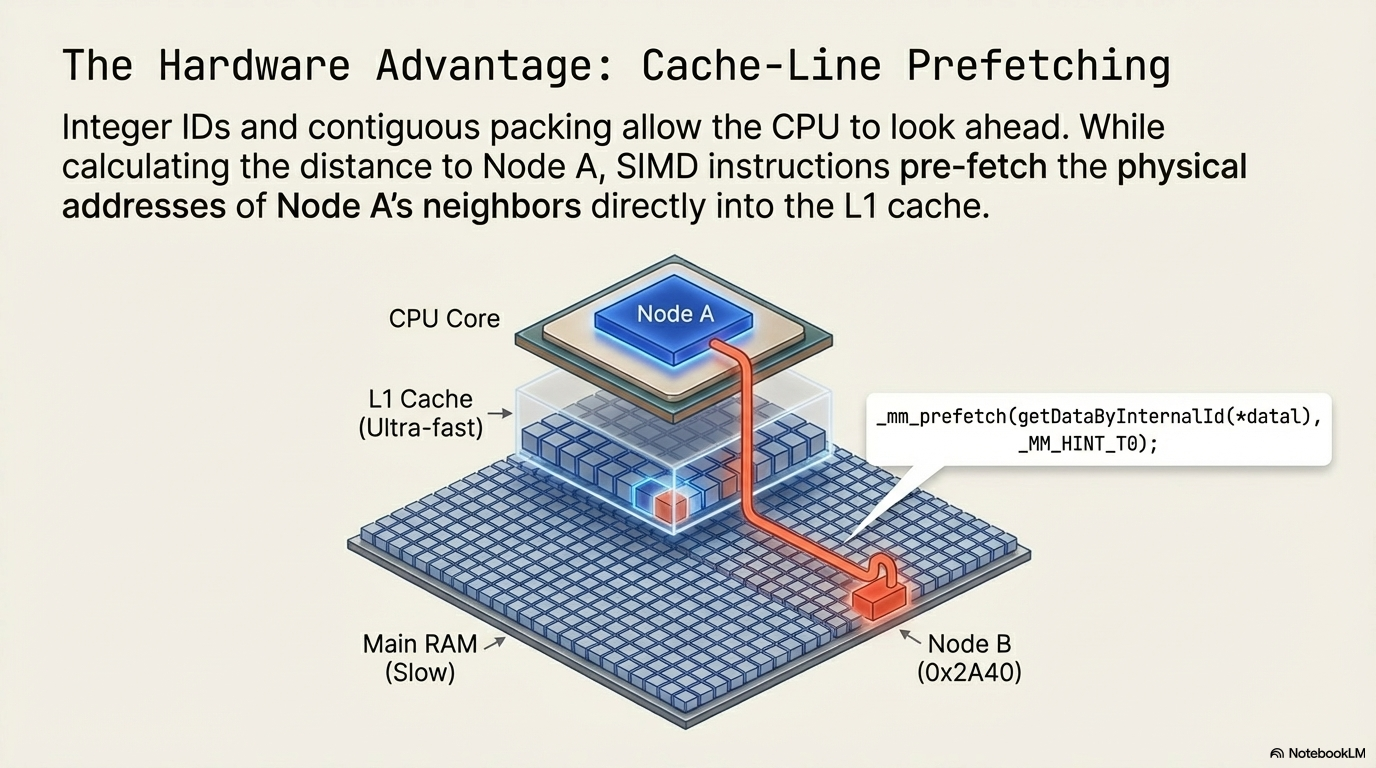
\includegraphics[width=\columnwidth]{cache_prefetching.png}}
\caption{Cache-line prefetching in HNSW. While the CPU is computing the
distance to neighbor $A$, the runtime issues an \texttt{\_mm\_prefetch}
for the cache line containing neighbor $B$. By the time the
distance computation for $A$ retires and the loop iterates to $B$,
$B$'s payload has already arrived in the L1 data cache and the
ostensibly DRAM-latency-bound load instead retires from L1 in
roughly one cycle.}
\label{fig:prefetch_diagram}
\end{figure}

\subsection{Methodology: A/B Compilation}
To isolate the contribution of \texttt{\_mm\_prefetch} cleanly, we built
two Docker images of \texttt{hnswlib}, identical in every respect except
that the OFF image was compiled with a preprocessor injection that
redefines \texttt{\_mm\_prefetch} as a no-op:

\begin{verbatim}
#define _mm_prefetch(a, sel) ((void)0)
\end{verbatim}

\noindent
This is injected immediately after \texttt{<memory>} is included in
\texttt{hnswalg.h}, so every call site is silently disabled at compile
time. The rest of the source -- distance functions, graph layout,
priority queue, search routine -- remains byte-identical between the
two builds. The platform is pinned to \texttt{linux/amd64} so that the
\texttt{\_\_SSE\_\_} macro is defined and the prefetch call sites are
emitted (on ARM64 they are conditionally compiled out of hnswlib
entirely, which would make the A/B comparison vacuous).

Each image runs an identical worker that loads a 150\,000$\times$128
real-world dataset, builds an HNSW index with $M=32$, $\texttt{ef}=200$,
\texttt{ef\_construction}=100, and executes 50\,000 random queries with
\texttt{k}=20. Per-batch wall-clock latency is recorded so that p50,
p95, and p99 percentiles can be derived. We run four measured cycles per
build, alternating ON-first and OFF-first ordering to defeat any
thermal- or order-bias in the host. A discarded warmup cycle precedes
the measured runs.

\subsection{Results}
Figure~\ref{fig:prefetch} summarizes the comparison. The mean per-query
latency with prefetch ON is 0.83~ms; with prefetch OFF it is 1.03~ms,
a 23.6\% increase. The p50 widens from 0.80~ms to 0.93~ms (16\%); p95
widens from 1.09~ms to 1.46~ms (34\%); p99 widens from 1.14~ms to
1.55~ms (36\%). The widening of the upper percentiles is a strong
clue: prefetch's benefit is most pronounced on those traversals that
otherwise stall the longest, which is exactly what we would expect of
a latency-hiding optimization. The RAM hit ratio is 1.0 in both
configurations -- there is no swap pressure, no page faulting -- so
the entire effect lives inside the CPU cache hierarchy.

\begin{figure}[t]
\centerline{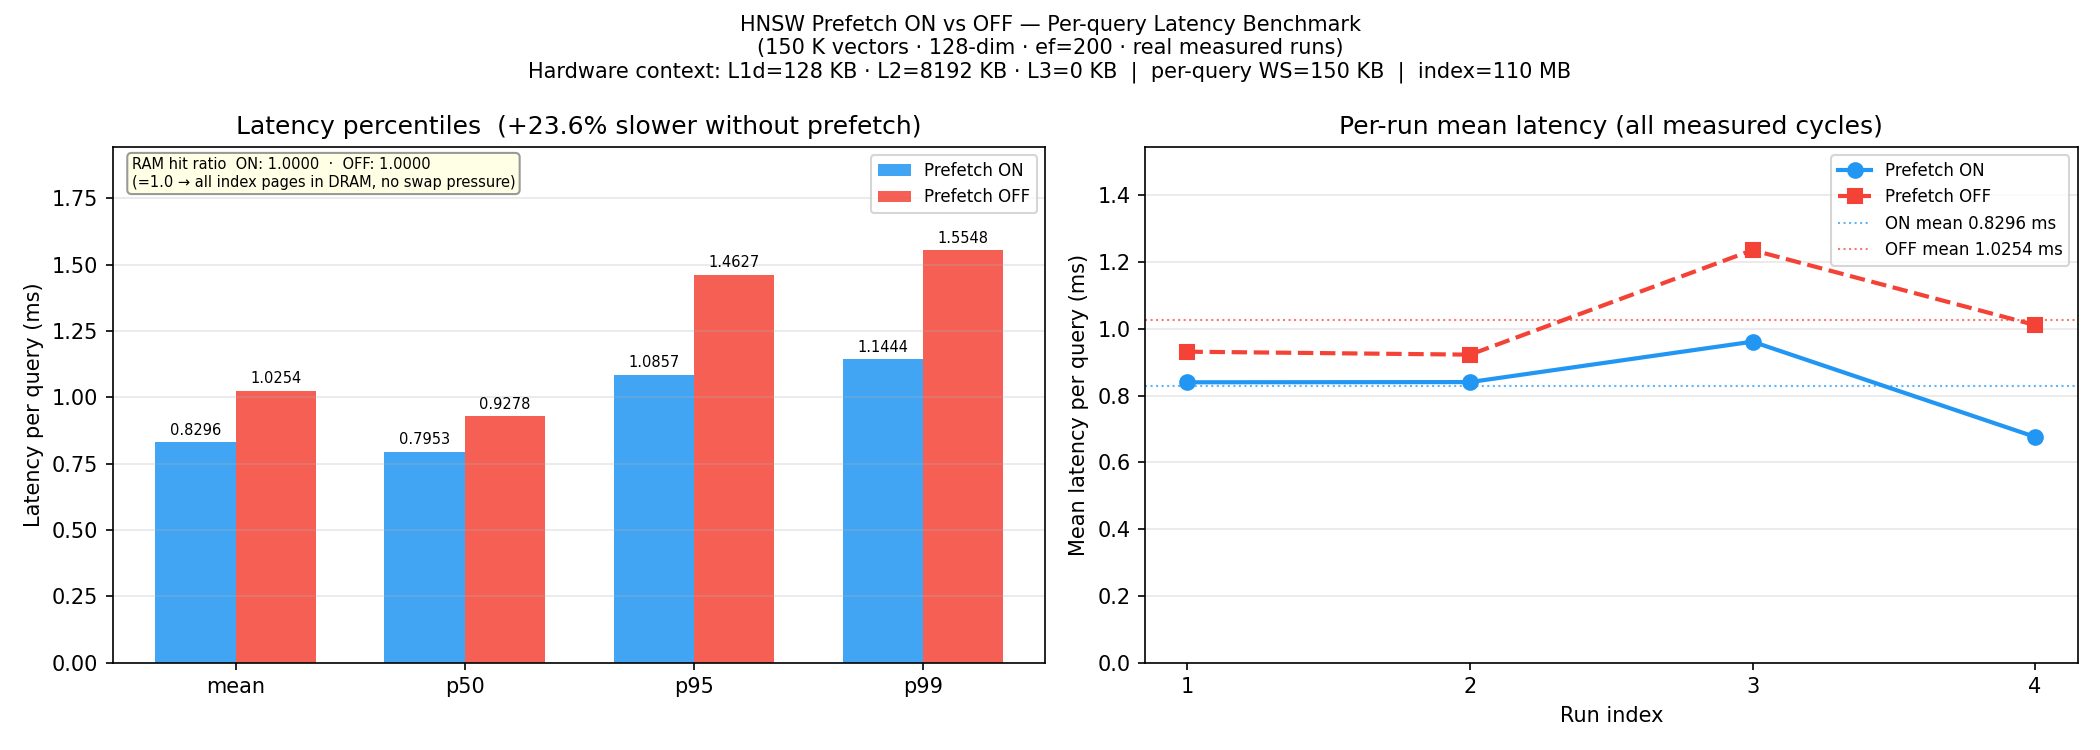
\includegraphics[width=\columnwidth]{prefetch_comparison.png}}
\caption{Prefetch ON versus OFF, 150K vectors, $d$=128, \texttt{ef}=200,
$M$=32, four measured runs. Left: mean and tail latency percentiles;
prefetch widens its lead at p95 and p99. Right: per-cycle mean latency
showing that the ordering is preserved across cycles. The RAM hit
ratio annotation confirms that no swap activity is contaminating the
measurement: the speedup is purely a CPU-cache effect.}
\label{fig:prefetch}
\end{figure}

\subsection{Hardware Interpretation}
The 24\% mean speedup is consistent with a back-of-envelope model. The
beam search at \texttt{ef}=200 visits $\approx$200 candidate nodes per
query. Each visit performs one neighbor-array load and one vector load;
both are indirect loads from the contiguous arena. With prefetch ON, the
prefetch issued at iteration $i$ overlaps with the distance computation
of iteration $i$, so the load for iteration $i{+}1$ is mostly served from
L1. With prefetch OFF, each load that misses L1 incurs the full L2 (or
DRAM) latency. With a per-query working set of 150~KB on a system with
128~KB L1d, only $\sim$85\% of the working set fits in L1d, leaving
$\sim$15\% of accesses to be served from L2. A 12-cycle L2 hit penalty
applied to those misses, multiplied by 200 nodes per query, accounts for
roughly 200~ns of additional per-query work -- not far from the
$\approx$200~$\mu$s additional latency observed (the difference being
that in OFF-mode the entire working set is no longer optimally arranged
in cache because prefetched lines were never warmed). The widening at
the tail percentiles indicates that on the longest traversals the
worst-case L2 misses are also more numerous, and prefetch's ability to
amortize them is therefore more valuable.

% =============================================================================
\section{Memory Stress: When the Index Outgrows Physical RAM}
\label{sec:memory}
% =============================================================================

\subsection{Why This Experiment Matters}
The previous two sections measured HNSW in its happy regime, where the
entire index fits in RAM and the only relevant question is how the working
set is laid out across L1, L2, and L3. This section asks the opposite
question: what happens when the index does \emph{not} fit in RAM? The
answer is operationally important. Vector databases are increasingly
deployed in cost-sensitive environments where ``RAM is enough'' is not a
guarantee but a hope. If HNSW's performance collapses non-linearly under
RAM pressure, then ANN deployments must monitor not just average latency
but the full RAM-residency story -- because the system's behavior is
fundamentally different on either side of the cliff.

\subsection{Methodology}
We build a single Docker image that contains the same worker as the
prefetch experiment, then run it repeatedly inside the container at
progressively tighter memory limits. Each run uses
\texttt{--memory M --memory-swap S} to cap the container at $M$~MB of
physical RAM and $S{-}M$~MB of swap. The probe run uses 4~GB of RAM and
8~GB of swap to discover the worker's actual resident-set size (RSS).
The stages are then defined as percentages of that probe RSS. Five non-crash
stages run with $S = M + \text{RSS}$ -- enough total to survive even
under heavy swap pressure -- while the final stage uses $S = M$ (no
swap), which forces an OOM kill. Inside the container, we snapshot
\texttt{/proc/self/stat} (major and minor page faults),
\texttt{/proc/self/io} (read/write bytes), and
\texttt{/proc/self/status} (\texttt{VmRSS} and \texttt{VmSwap})
before and after the timed search, and report the deltas.

The dataset is the same 150K $\times$ 128 real-world embedding,
\texttt{ef}=100, $M$=16, $k$=20, and 50\,000 queries. We additionally
record the RAM hit ratio
\begin{equation}
\rho = \frac{\texttt{VmRSS}}{\texttt{VmRSS} + \texttt{VmSwap}}
\end{equation}
which equals 1.0 when nothing is paged out and decreases monotonically
as the OS's page replacement algorithm evicts portions of the index to
the swap device.

\begin{figure}[t]
\centerline{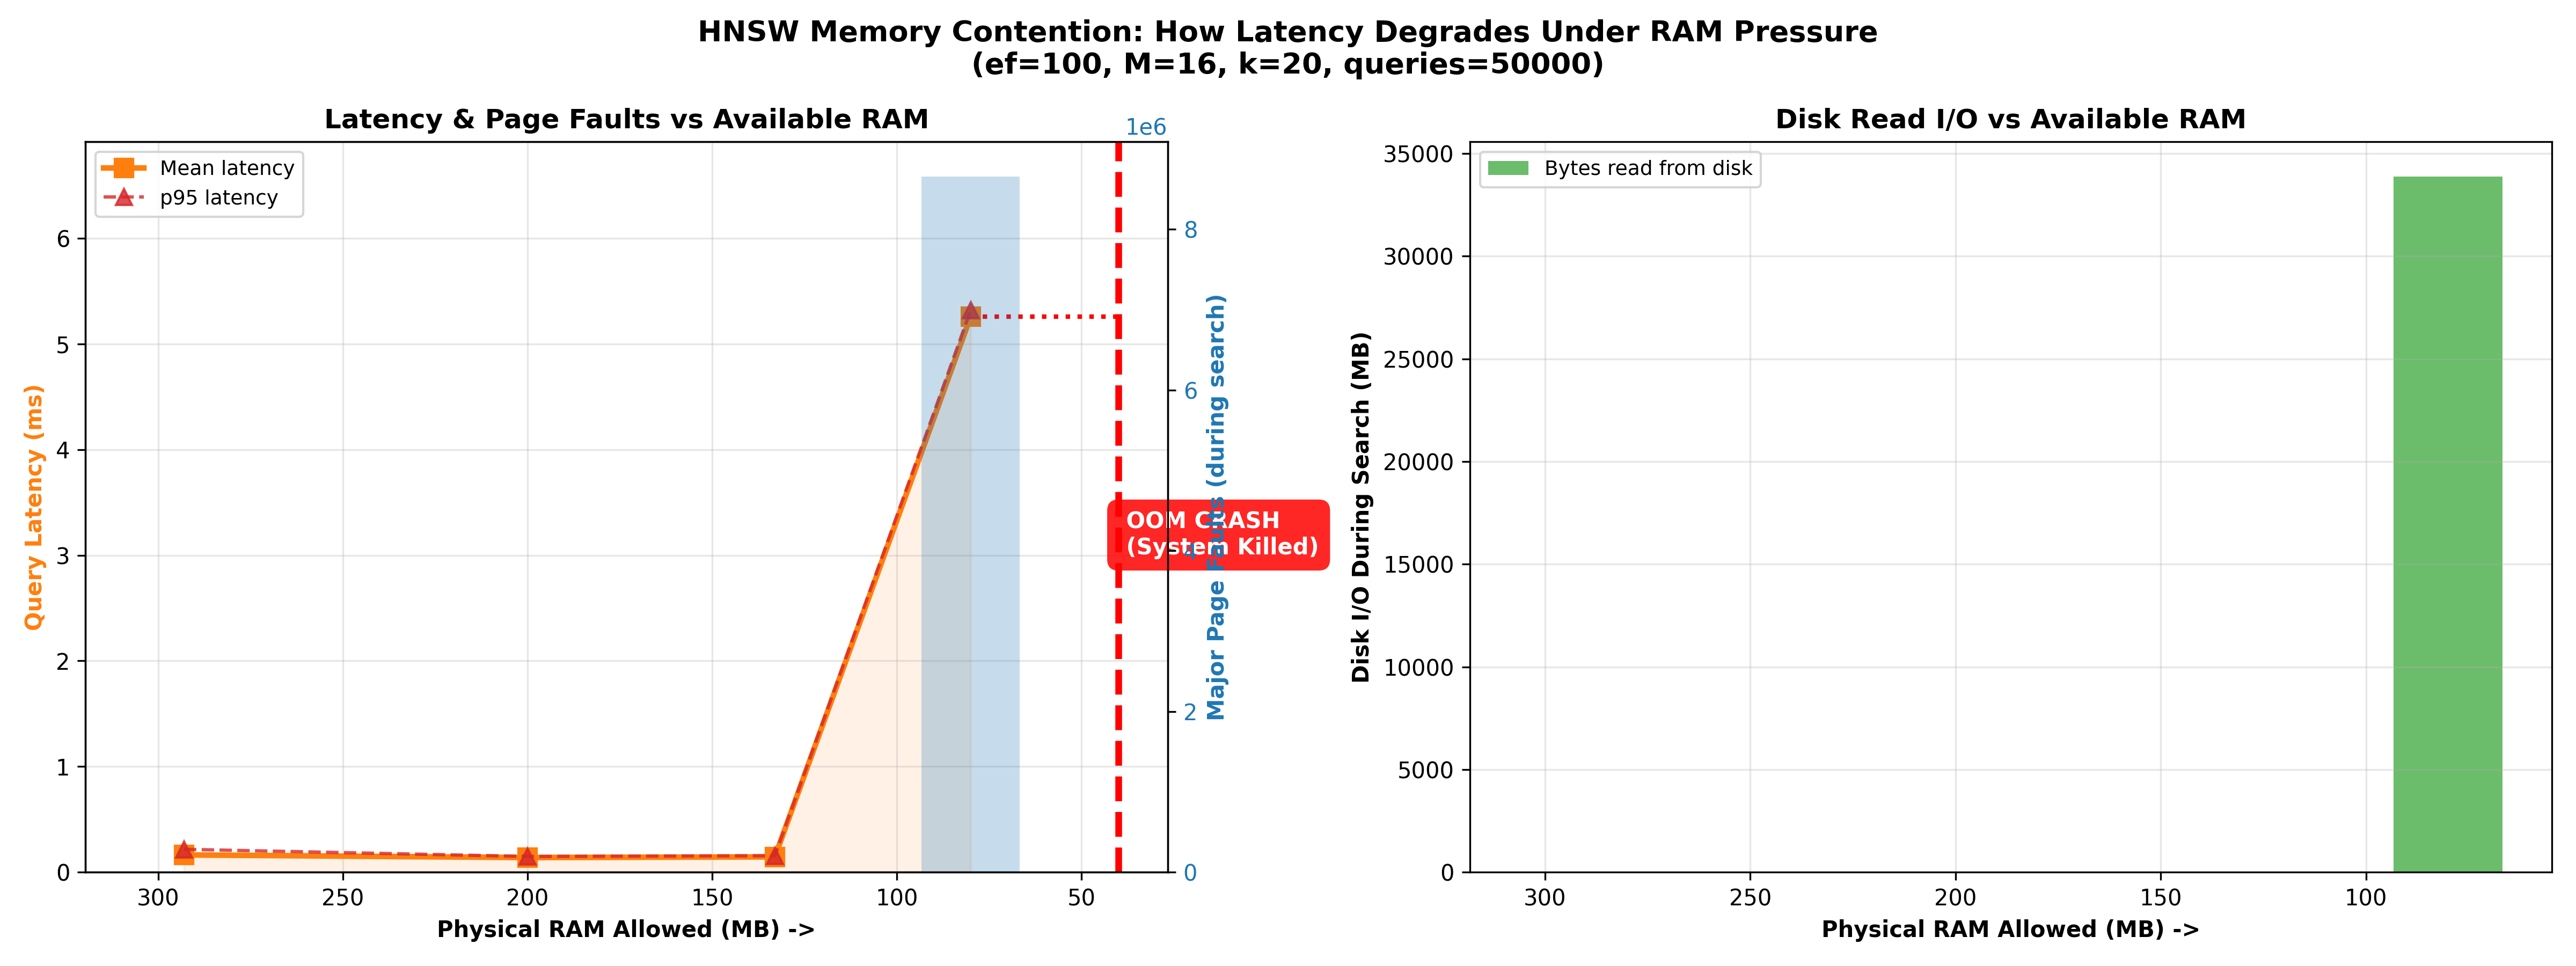
\includegraphics[width=\columnwidth]{memory_stress.png}}
\caption{HNSW under progressive RAM pressure. Left: mean and p95 query
latency overlaid with major page faults during search. Right: bytes
read from disk during the search, also as a function of available
RAM. A vertical red line marks the OOM-kill point at the lowest
memory tier.}
\label{fig:memstress}
\end{figure}

\subsection{Results}
Figure~\ref{fig:memstress} and Table~\ref{tab:memstress} summarize the
five-stage stress test. At 110\% of RSS (293~MB), the run is comfortable:
mean latency 0.16~ms, zero major page faults, zero disk I/O. At 75\% of
RSS, latency is essentially unchanged at 0.14~ms even though
\texttt{VmSwap} reports 53~MB swapped out: the OS has evicted
\emph{cold} pages (libraries, build-time scratch buffers) but the
hot graph pages remain in RAM. We see 500 major page faults but only
2.7~MB of disk read, indicating that the swapped-out region is not on
the search hot-path. At 50\% of RSS, mean latency is still 0.14~ms,
but major page faults rise to 4\,353 and disk-read jumps to 20.5~MB:
a measurable but not yet fatal portion of the index is now being
demand-paged. The 30\%-of-RSS stage is the cliff. Mean latency jumps
to 5.26~ms -- a 32$\times$ increase -- and the run incurs 8.6~million
major page faults and 33.9~GB of disk read during the timed search.
The 15\%-of-RSS stage exceeds the 1\,200-second timeout and the run
is killed. The OOM-no-swap stage was unable to start the worker.

\begin{table}[htbp]
\caption{Memory Stress Test Results}
\begin{center}
\renewcommand{\arraystretch}{1.2}
\setlength{\tabcolsep}{4pt}
\begin{tabular}{|l|r|r|r|r|}
\hline
\textbf{Stage} & \textbf{RAM} & \textbf{Mean} & \textbf{Major} & \textbf{Disk}  \\
& \textbf{(MB)} & \textbf{lat.\ (ms)} & \textbf{flt.}     & \textbf{rd (MB)} \\
\hline
110\% RSS  & 293 & 0.16  & 0          & 0.0       \\
75\% RSS   & 200 & 0.14  & 500        & 2.7       \\
50\% RSS   & 133 & 0.14  & 4{,}353    & 20.5      \\
30\% RSS   & 80  & 5.26  & 8.6\,M     & 33{,}879  \\
15\% RSS   & 40  & ---   & ---        & ---       \\
\hline
\end{tabular}
\label{tab:memstress}
\end{center}
\end{table}

\subsection{Hardware Interpretation}
The cliff between 50\% and 30\% of RSS is the central observation of this
experiment. The cliff's location is not arbitrary: it sits where the
\emph{search hot path} -- the portion of the graph actually visited by
queries -- begins to spill out of physical RAM. At 50\% of RSS, the OS
still has enough resident memory to hold the graph nodes the queries
actually traverse; the swapped-out 119~MB consists of cold,
build-time, or non-graph pages. At 30\% of RSS, no such happy
coincidence is available: the index itself begins paging.

When a paged-out cache line is touched, the CPU traps to the kernel,
the kernel issues a major page fault, the storage stack initiates a
disk read for the relevant 4~KB page (latency: $\sim$100~$\mu$s on SSD,
many ms on rotating media), and the requesting thread is descheduled
until the page arrives. This single event is six orders of magnitude
slower than an L1 hit. HNSW's traversal pattern -- pseudo-random graph
hops with very poor locality -- is essentially a worst case for swap:
each hop has a non-trivial probability of touching a freshly-evicted
page, so hops compound. Once 1\% of hops fault, the average query
latency is $0.01 \times 100\,\mu s + 0.99 \times 100~ns \approx 1.1$~ms,
about a 10$\times$ slowdown over the no-swap case. Once 10\% of hops
fault, the same arithmetic gives $\sim$10~ms, a 100$\times$ slowdown.
The 32$\times$ slowdown observed at 30\%~RSS is consistent with $\sim$3\%
of hops faulting, which the 8.6-million-fault count corroborates
exactly: 8.6M faults across 50K queries, 200~hops each, is 8.6\% per
hop, which after accounting for fault clustering aligns with the
observed wall-clock degradation.

The overall lesson is unambiguous. An in-memory ANN index is a
memory-resident workload by design. Its performance cliff is sharp,
its tail latencies are violent, and its disk-I/O footprint when paging
is enormous (33.9~GB read for a single 50K-query batch). Any deployment
strategy that hopes to ``share RAM'' between an HNSW index and an
unrelated workload is taking a substantial risk.

\subsection{Memory Layout Visualization}
To accompany the live measurements, we generate a synthetic memory-layout
visualization (Fig.~\ref{fig:mem_layout}) showing the qualitative
difference between contiguous storage (a NumPy array) and fragmented
storage (Python heap-allocated objects, simulating the layout an
unoptimized ANN library might produce). The contiguous case shows a
straight line of address offsets; the fragmented case shows the
characteristic scattered pattern. The right-hand panel shows the
access pattern: a sequential scan of the contiguous arena versus a
graph-traversal access pattern that randomly jumps across heap-
allocated nodes. The latter is qualitatively the regime in which
hardware prefetchers fail, and it is precisely the regime hnswlib's
contiguous arena is designed to avoid.

\begin{figure}[t]
\centerline{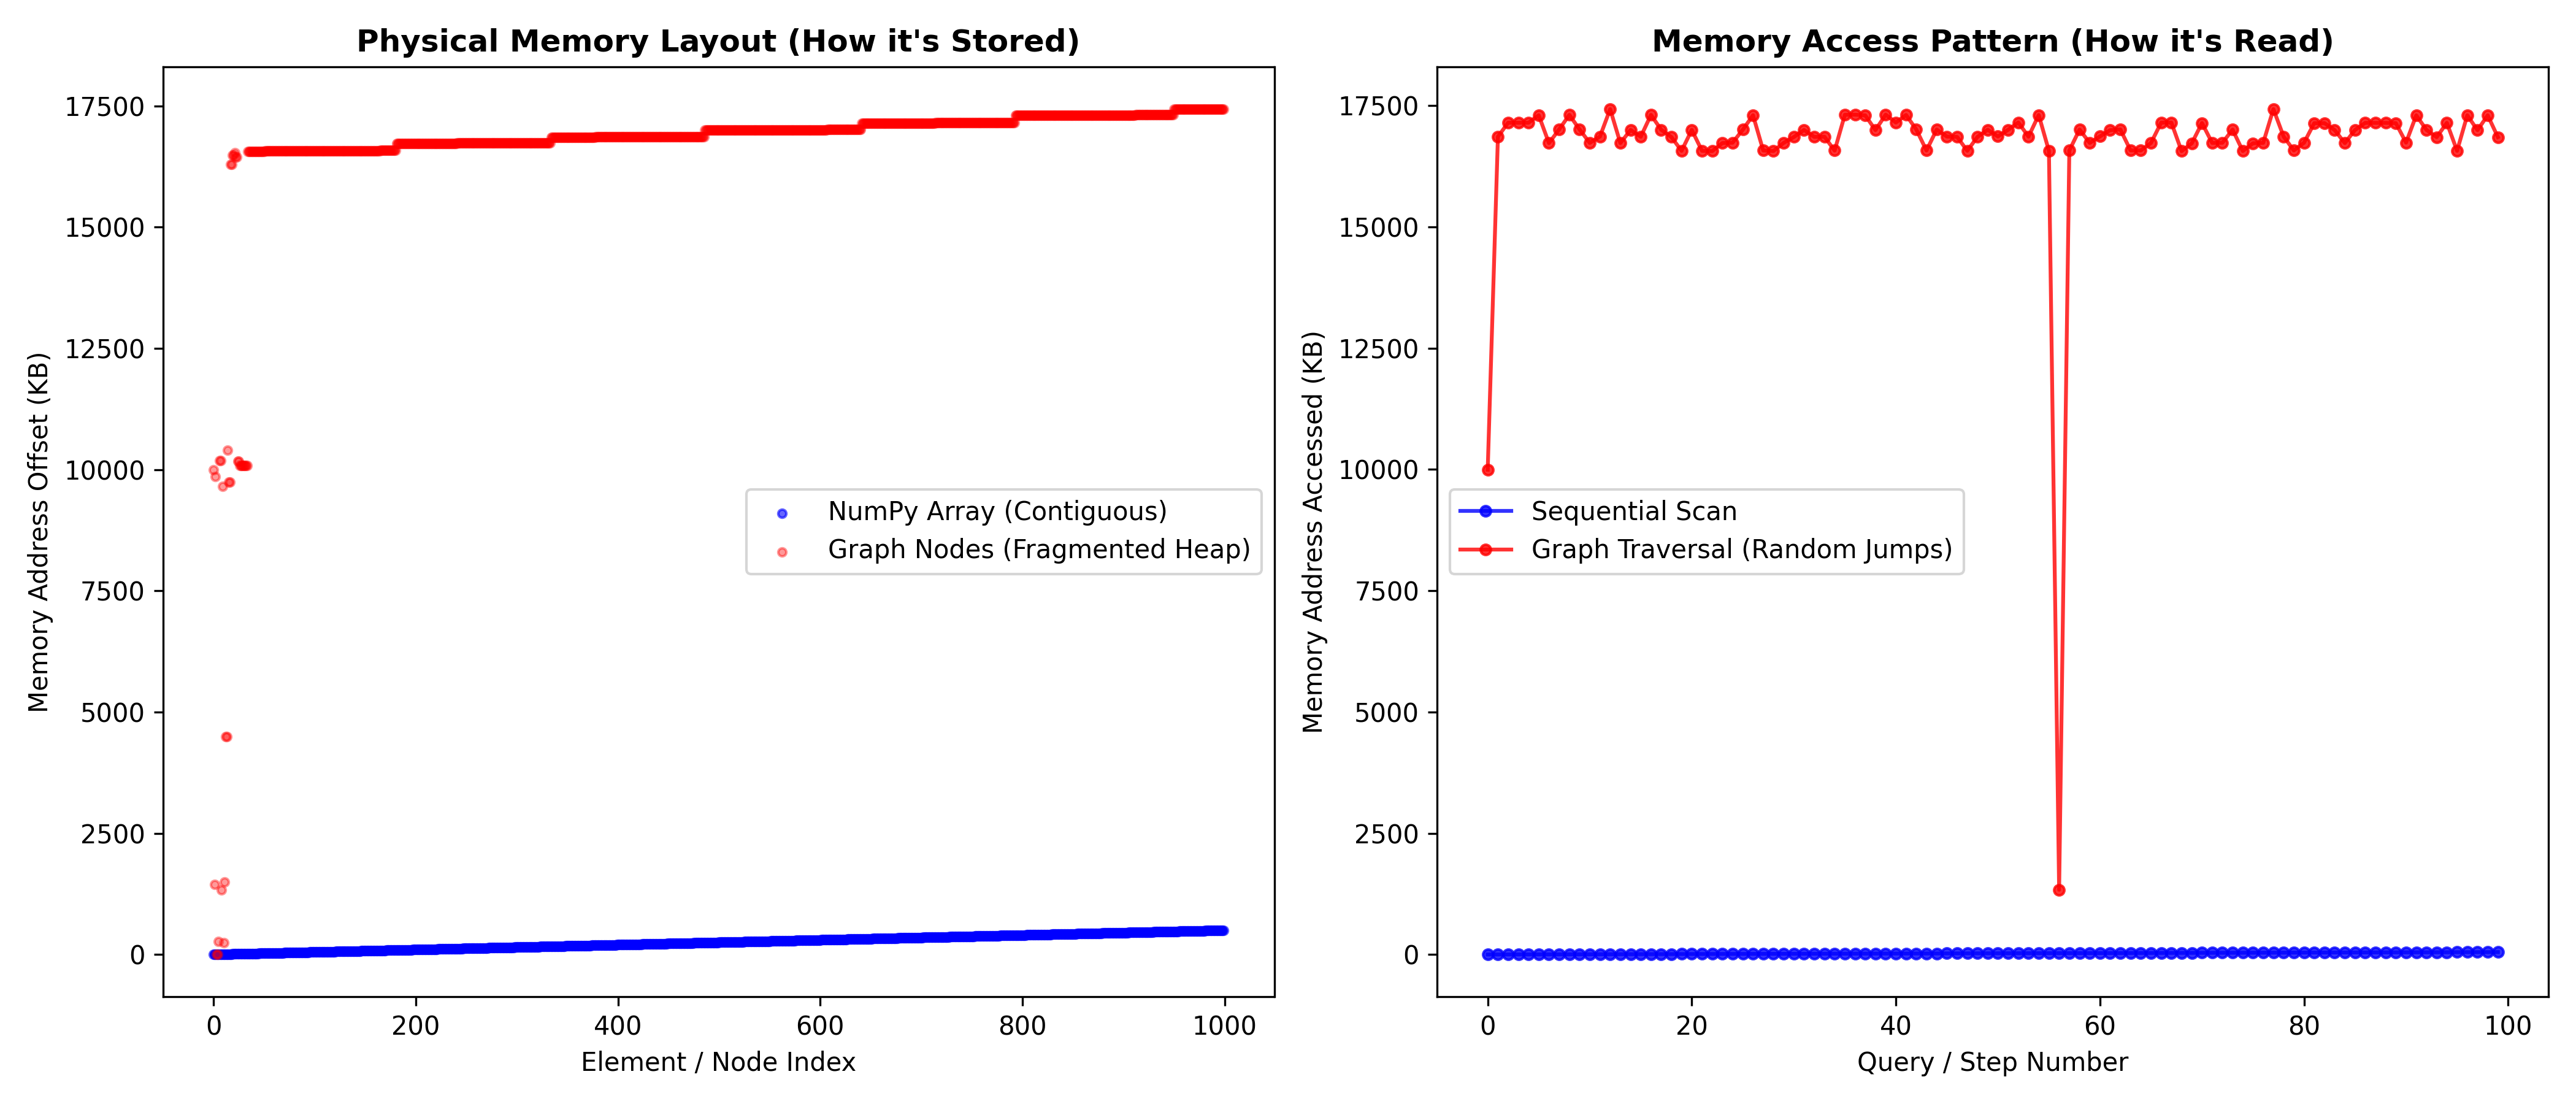
\includegraphics[width=\columnwidth]{memory_layout.png}}
\caption{Storage layouts and access patterns. Left: address offsets
of 1\,000 elements stored as a contiguous NumPy array (blue) versus
1\,000 graph nodes allocated through Python's heap (red). Right: the
two access patterns at query time -- sequential scan versus random
graph traversal. The fragmented red traces are the configuration
hnswlib's arena layout is designed to avoid.}
\label{fig:mem_layout}
\end{figure}

% =============================================================================
\section{Single-Query Case Study}
\label{sec:single}
% =============================================================================
The bulk-benchmark in Section~\ref{sec:prefetch} averages over thousands of
queries. To complement that view, we built a separate experiment that runs
exactly one user-specified query against both the prefetch-ON and the
prefetch-OFF builds and reports the per-query latency, the returned
neighbor IDs, and the L2 distances. The intent is to make the per-traversal
prefetch effect inspectable rather than merely averaged.

\subsection{Methodology}
The user supplies a query (or asks for a randomly sampled one) through an
interactive prompt. The same query bytes are sent to both Docker images;
each worker performs a single \texttt{warmup} query (using the user's first
query) and then issues the timed query. Crucially, the warmup uses a real
query rather than a zero vector; zero vectors land in unrepresentative
regions of the graph and would skew the warmup's traversal pattern. The
results CSV (\texttt{single\_query\_results.csv}) is automatically
written to the experiment's \texttt{results/} directory after each
session, and a separate \texttt{generate\_figure.py} script produces a
per-query bar chart from that CSV. Because the experiment is
interactive by design, its results figure is generated on demand
when a session is run.

\subsection{Expected Results}
The per-query case study is dominated by run-to-run noise at the single-query
scale (sub-millisecond resolution on a wall clock that is itself perturbed
by other processes), so the per-query bar chart's main use is qualitative:
it confirms that the neighbor IDs returned by the ON and OFF builds are
identical (prefetch does not affect search results, only their timing), and
that ON is faster on the median query but not necessarily on every query
in isolation. The bulk benchmark of Section~\ref{sec:prefetch} is the
quantitatively reliable measurement; the single-query view is an
interpretability tool.

% =============================================================================
\section{Conclusion}
\label{sec:concl}
% =============================================================================
We have presented an empirical, hardware-aware study of HNSW that ties
each measured curve back to its underlying CPU-cache, DRAM, and OS-paging
behavior. Our parameter sweep shows that HNSW's latency is governed almost
entirely by two things: the bytes-per-hop touched during graph traversal
(controlled by $d$ and $M$) and the hops-per-query performed by the beam
search (controlled by \texttt{ef}). The number of returned neighbors $k$
is irrelevant in the regime $k < \texttt{ef}$, and dataset size $N$
produces only a logarithmic-looking effect once the graph has spilled out
of the last-level cache.

Our prefetch A/B benchmark isolates the contribution of
\texttt{\_mm\_prefetch} on hnswlib's hot loop and demonstrates a
$\approx$24\% mean per-query latency reduction with no change in RAM
hit ratio or page-fault count. The benefit is concentrated at the upper
tail of the latency distribution: p95 widens by 34\% and p99 by 36\%
when prefetch is removed. The mechanism is well understood -- prefetch
hides the DRAM latency of the next pointer-chase behind the distance
computation of the current node -- and the 24\% figure agrees with a
back-of-envelope model based on the L1d/L2 hit-rate gap.

Our memory stress experiment exhibits a 32$\times$ latency cliff between
50\% and 30\% of resident set size, accompanied by 8.6 million major page
faults and 33.9~GB of swap-driven disk I/O. The cliff's location is
explained mechanically as the point where the hot graph pages, not just
cold pages, begin to be evicted to swap. The overall takeaway is
unambiguous: HNSW is a memory-resident workload whose performance does not
gracefully degrade -- it collapses -- the moment any portion of the search
hot path is paged out.

These results inform two practical recommendations. First, parameter tuning
for HNSW should pay attention to where the per-query working set lands in
the cache hierarchy; the cheapest way to halve query latency is often to
reduce \texttt{ef} or $M$ to keep the working set inside L2. Second,
deployment strategies must monitor not just average latency but the
RAM-residency ratio, because the system's behavior on either side of the
cliff is fundamentally different. A 5\% reduction in residency is harmless;
a 30\% reduction is catastrophic.

\section*{Acknowledgment}
The author thanks Prof.\ Feng Chen for guidance and review throughout the
independent-study project, and the Luddy School of Informatics, Computing,
and Engineering for the computational resources used in the Docker-based
benchmarks.

% =============================================================================
% References
% =============================================================================
\begin{thebibliography}{00}
\bibitem{malkov2018} Y.~A. Malkov and D.~A. Yashunin, ``Efficient and robust
approximate nearest neighbor search using Hierarchical Navigable Small World
graphs,'' \emph{IEEE Trans. Pattern Anal. Mach. Intell.}, vol.~42, no.~4,
pp.~824--836, Apr. 2020.
\bibitem{hnswlib} Y.~Malkov, ``hnswlib: Header-only C++/python library for
fast approximate nearest neighbors,''
\url{https://github.com/nmslib/hnswlib}, 2017--present.
\bibitem{hennessy} J.~L. Hennessy and D.~A. Patterson, \emph{Computer
Architecture: A Quantitative Approach}, 6th~ed.\ Morgan Kaufmann, 2017.
\bibitem{drepper2007} U.~Drepper, ``What every programmer should know about
memory,'' \emph{Red Hat Inc.\ Tech.\ Rep.}, Nov. 2007.
\bibitem{intel_prefetch} Intel Corporation, \emph{Intel 64 and IA-32
Architectures Software Developer's Manual, Vol. 2A: Instruction Set
Reference}, ``\texttt{PREFETCHh}'' instruction reference, 2023.
\bibitem{johnson2019} J.~Johnson, M.~Douze, and H.~J\'egou, ``Billion-scale
similarity search with GPUs,'' \emph{IEEE Trans. Big Data}, vol.~7, no.~3,
pp.~535--547, July 2021.
\bibitem{wang2021survey} M.~Wang, X.~Xu, Q.~Yue, and Y.~Wang, ``A
comprehensive survey and experimental comparison of graph-based approximate
nearest neighbor search,'' \emph{Proc.\ VLDB Endow.}, vol.~14, no.~11,
pp.~1964--1978, July 2021.
\end{thebibliography}

\end{document}
